\section{Strided and Offset Memory Access (3 Points)}

\subsection{Task a}
\begin{figure}[h]
    \begin{center}
        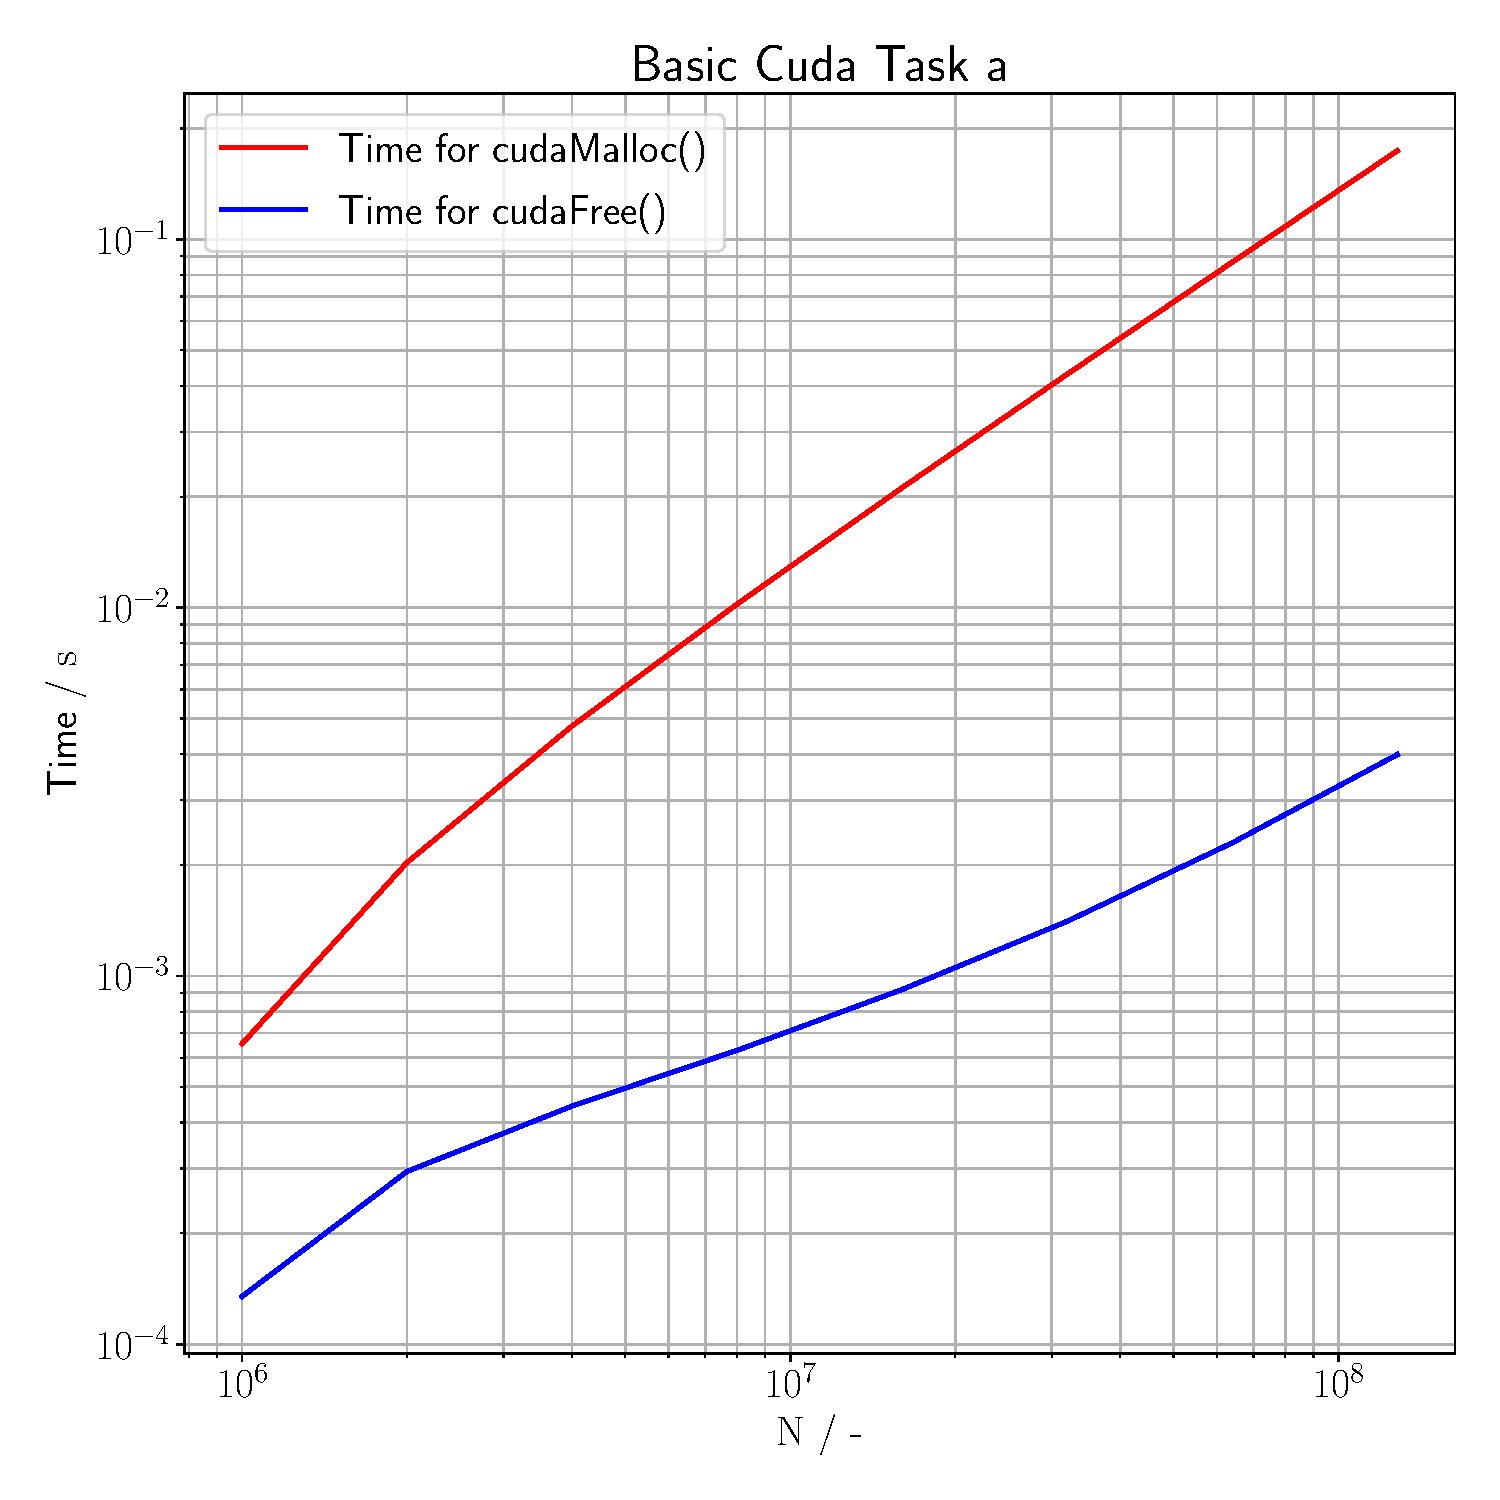
\includegraphics[width=1\textwidth]{figures/task_1_a.pdf}
        \caption{Plot for task 1a - see code in appendix \ref{app_1a}}
        \label{task_1_ab_plot}
    \end{center}
\end{figure}
\pagebreak

\subsection{Task b}
\begin{figure}[h]
    \begin{center}
        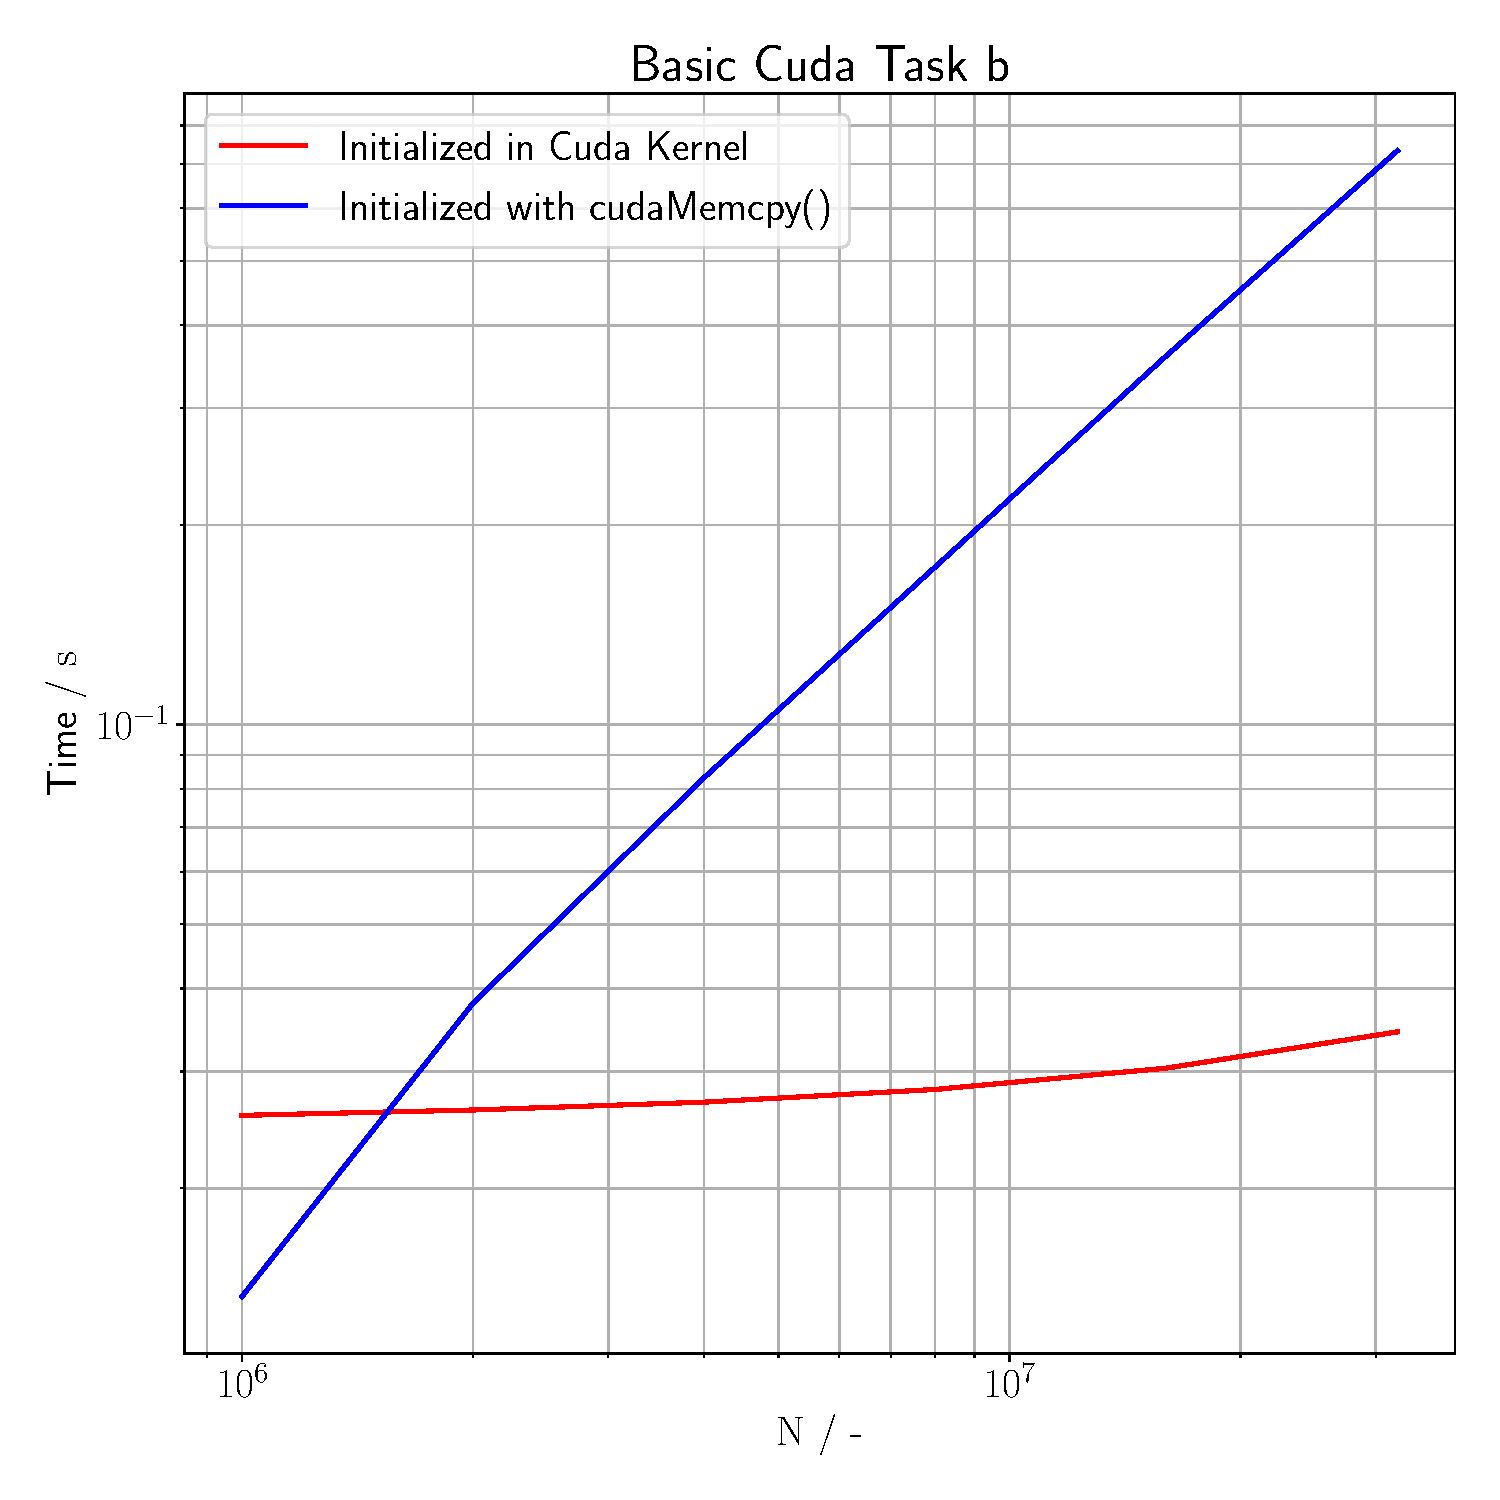
\includegraphics[width=1\textwidth]{figures/task_1_b.pdf}
        \caption{Plot for task 1b - see code in appendix \ref{app_1b}}
        \label{task_1_b_plot}
    \end{center}
\end{figure} 
\pagebreak

\usetikzlibrary {graphs,quotes}
\tikz
  \graph [edge quotes={fill=white,inner sep=1pt},
          grow down, branch right, nodes={circle,draw}] {
    "" -> h [>"9"] -> {
      c [>"4"] -> {
        a [>"2"],
        e [>"0"]
      },
      j [>"7"]
    }
  };